\documentclass[10pt,times,twocolumn]{article}

\usepackage{sbcm2021}
\usepackage{graphicx,url}

% -------------------------------------------------------
% Packages that facilitate double-blind peer review
% Comment the first line and uncomment the second to remove double-blindness
%\usepackage[blind]{anonymize} % Blind
\usepackage{anonymize} % not blind
% --------------------------------------------------------

%\usepackage[brazil]{babel}
%\usepackage[latin1]{inputenc}
% If needed, change this to:
 \usepackage[utf8]{inputenc}


\sloppy

\title{Sample Document Using the \LaTeX\ Style for SBCM 2021}

\author{\anonymize{First Author}\inst{1}\thanks{Supported by \anonymize{CAPES}.} \and
        \anonymize{Second Author}\inst{1}\inst{2}}

\address{\anonymize{First Laboratory -- First School/Institute/University}\\
         \anonymize{Av. Prof. Luciano Gualberto, 158, tv. 3 -- 05508-900 Sao Paulo, SP}
         \nextinstitute
         \anonymize{Second Laboratory -- Universidade Federal de Pernambuco} \\
         \anonymize{Caixa Postal 15064 --90501-970 Recife, PE}
         \email{\anonymize{first\_email@poli.usp.br, second\_email@cin.ufpe.br}}
}


\begin{document}

\maketitle

\begin{abstract}
This meta-paper describes the style to be used in papers for SBCM 2021.
Full papers must be written in English. Short papers can be written in English, Portuguese, or Spanish.
Full papers, Art submission and posters must be anonymous for double-blind peer review; The abstract (in full papers) must be an objective text between 150 and 200 words clearly stating the contributions of the work.
Extended abstracts are not divided into sections, hence they do not need an abstract.
This template is based on the default conference template for SBC 2003.
\end{abstract}


\section{General Information: Full papers}\label{sec:gen}

All full papers submitted to SBCM 2021 must be written in English, and must be anonymous for double-blind peer review. The paper must be formatted to A4 paper, two columns, 2 cm top margin, 1.9 cm left and right
margin, 2.5 cm bottom margin and 0.81 cm separation between columns. Full papers must be between 4 and 8 pages long. Extended abstracts must be shorter than two pages. The main font should be Times New Roman, 10 pt.

\section{First Page}

The first page must display the paper title, the name and address of the authors (only in the camera-ready version), and the abstract in English. The title must be centered over the whole page, 16 points boldface font. Author names in the camera-ready version must be centered, 10 points font, boldface, all of them disposed in the same line, separated by commas. Addresses must be centered, 10 points font.
The abstract must be 10 points font, indented 0.8cm on both sides.

\section{Sections and Paragraphs}
Section titles must be in boldface, 13pt, flush left. There should be 10pt of extra space before each title. Section numbering is mandatory. All paragraphs must be indented by 1 cm.

\subsection{Subsections}

The subsection titles must be in boldface, 10pt, flush left.

\subsubsection{Subsubsection}

Subsubsections titles must be in boldface, 10pt, flush left.


\section{Figures and Captions}

Figures and tables captions should be centered if less than one line
(Figure~\ref{fig:exampleFig}), otherwise justified and indented by
0.8cm on both margins. The font must be Helvetica, 10 point, boldface,
with 6 points of space before and after each caption.

In tables, do not use colored or shaded backgrounds, and avoid thick,
doubled, or unnecessary framing lines. When reporting empirical data,
do not use more decimal digits than warranted by their precision and
reproducibility.

\begin{figure}[h]
\centering
  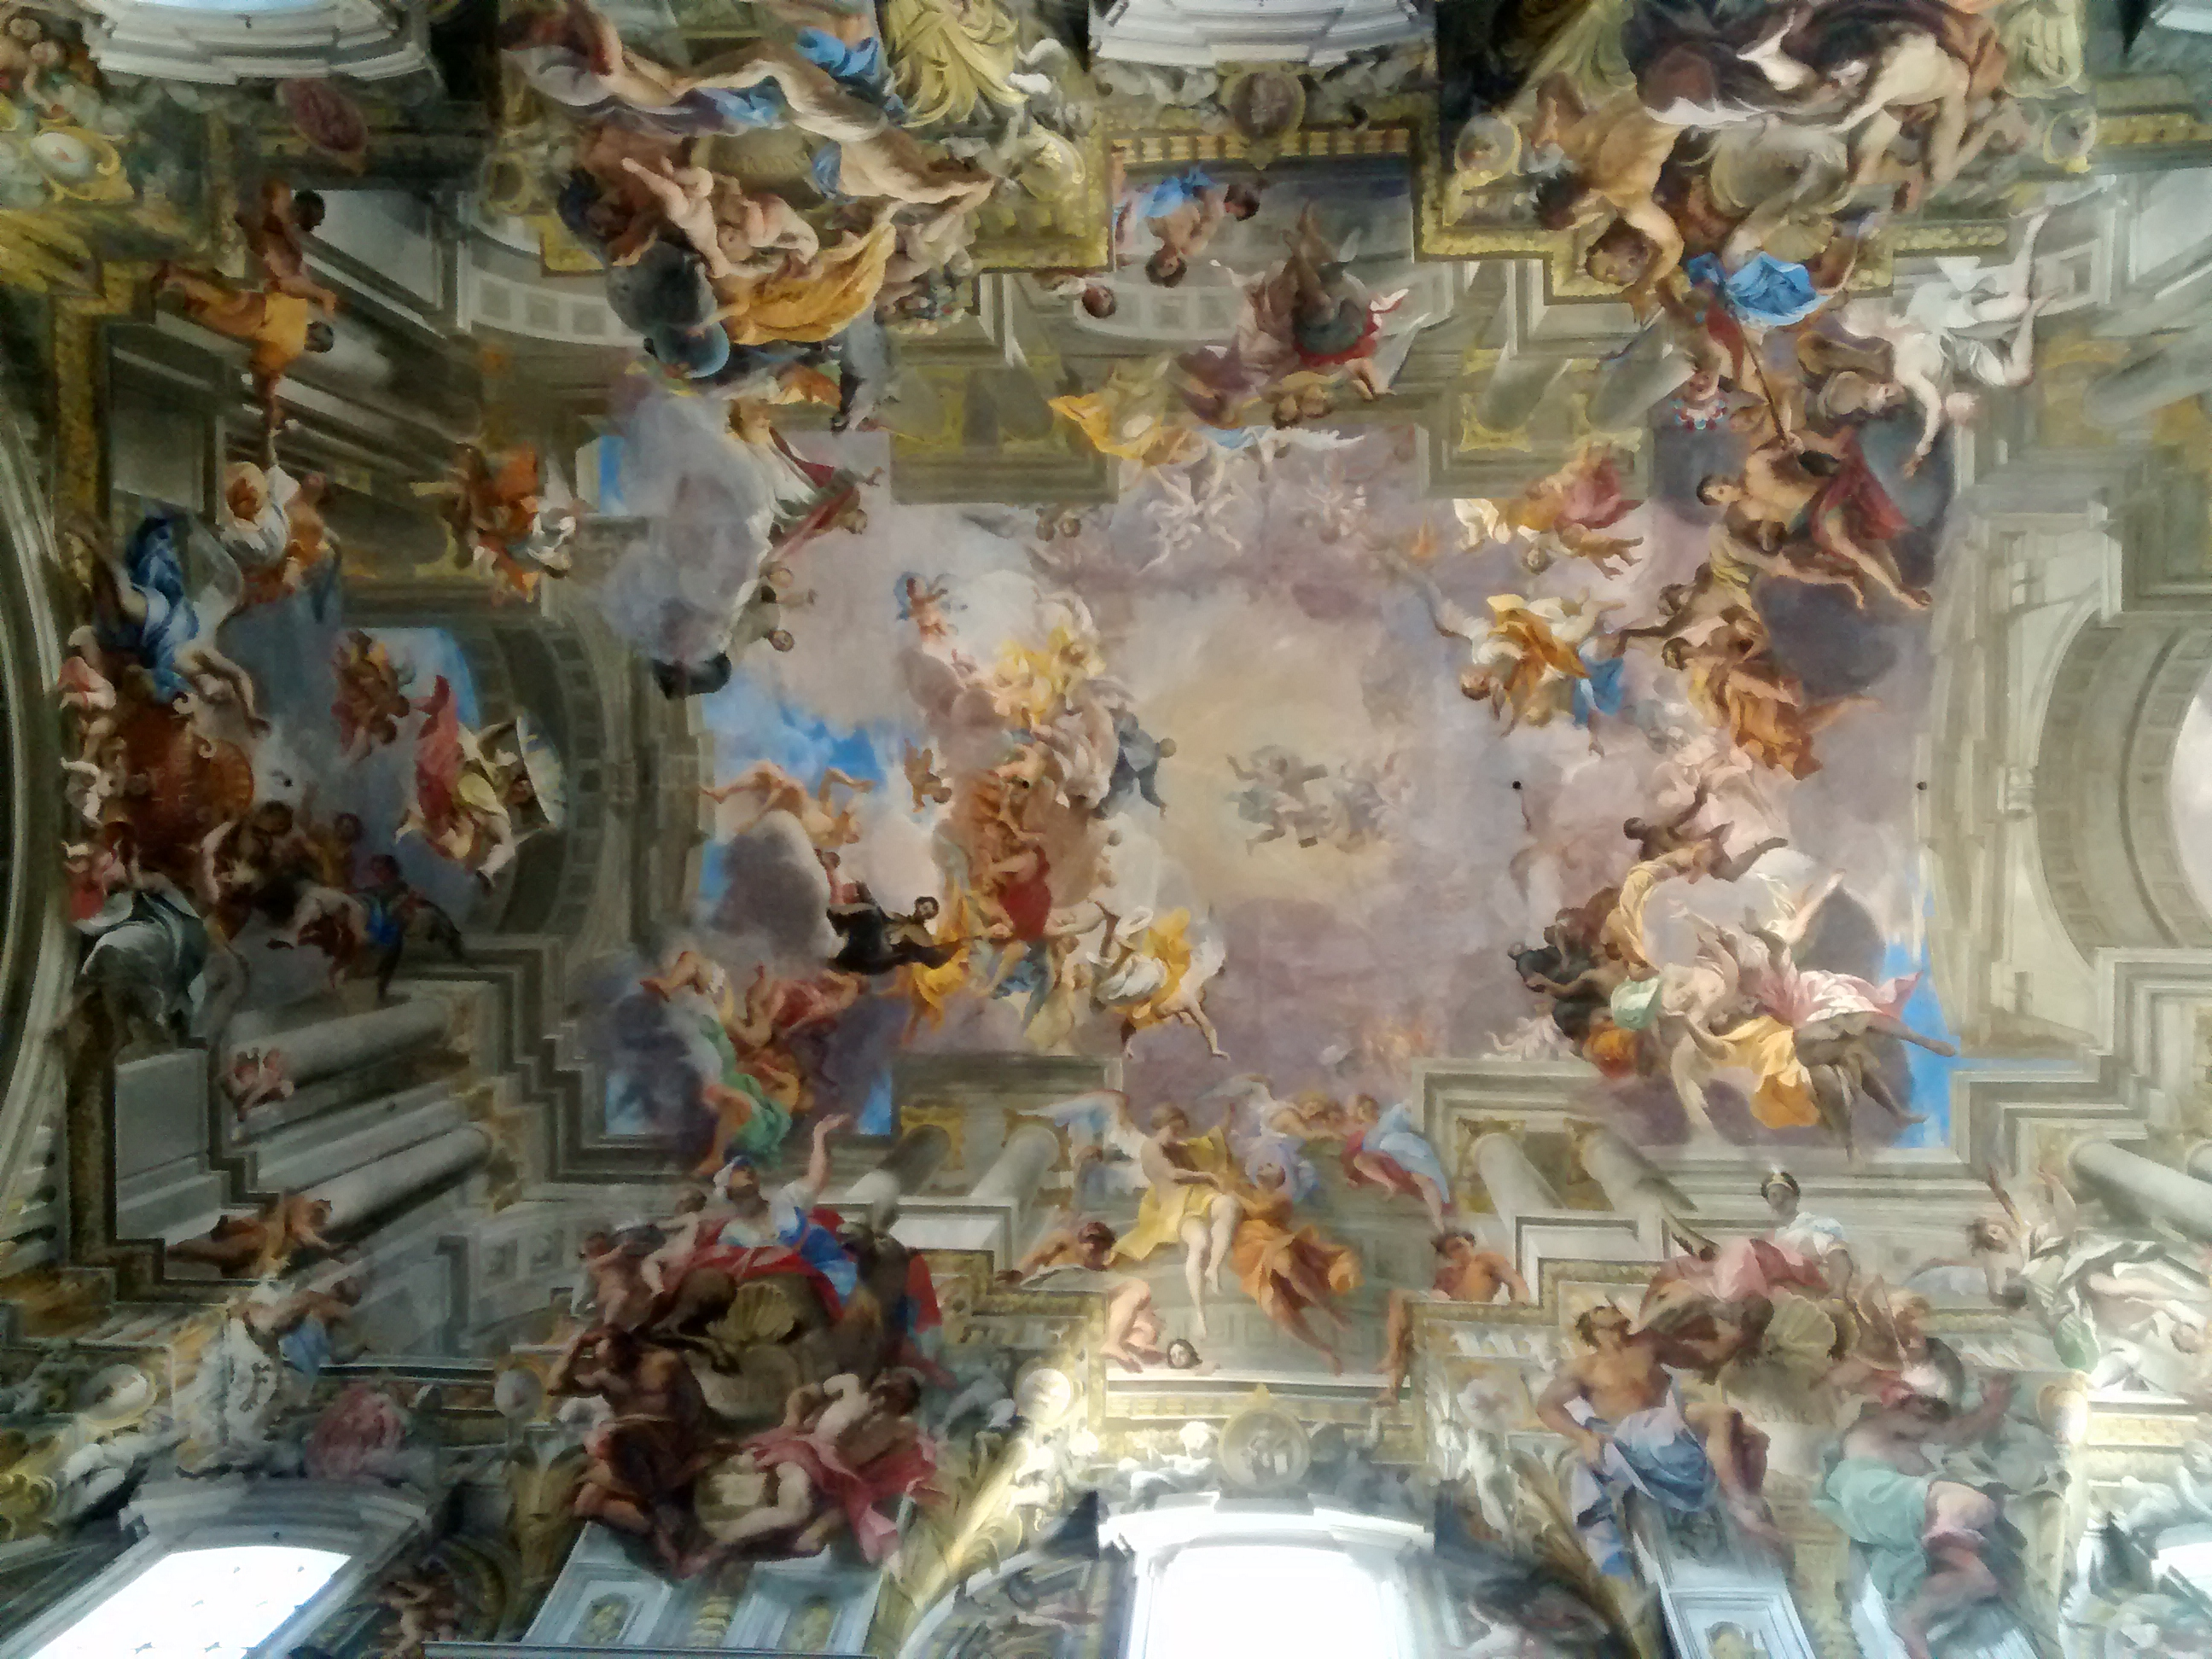
\includegraphics[width=.5\textwidth]{fig/ceiling.jpg}
\caption{A typical figure}
\label{fig:exampleFig}
\end{figure}


\section{Images}

All images and illustrations can be in color, but they must be visible in black-and-white, or gray tones.
The image resolution on paper should be about 600 dpi for black-and-white images, and 150--200 dpi for grayscale images. Do not include images with excessive resolution, as they may take hours to print, without any visible difference in the result.

\section{References}

Bibliographic references must be unambiguous and uniform. They must be numbered in order of appearance, e.g. \cite{knuth:89}, \cite{smith:99}.
Self-citations can be anonymized using the model \cite{\anoncite{Lamport:LaTeX}} or use constructions as: ``previous work by Author et al.'' instead of: ``our previous
work''.
If you need to cite the name of a \anonymize{tool}, \anonymize{website}, \anonymize{research group},
\anonymize{city}, or any other reference that can identify you, please, make it anonymous to double blind
review.


\bibliographystyle{unsrt}
\bibliography{example}

\end{document}

